\chapter{Specyfikacja komponentów interfejsu do rozpoznawania emocji}
\label{cha:specyfikacja}
Celem pracy jest opracowanie prototypu interfejsu umożliwiającego pomiar sygnałów pozwalających na określenie zmian stanów emocjonalnych gracza. W~związku z~tym na jeden z~elementów niniejszej pracy składa się przegląd możliwych rozwiązań użytych w~poszczególnych komponentach interfejsu. W~tym rozdziale skupiono się głównie na przedstawieniu urządzeń do pomiaru sygnałów umożliwiających określenie stanu emocjonalnego użytkownika, mechanizmach wnioskowania, które mogą zostać użyte podczas budowania modelu do rozpoznawania emocji, oraz silnikach do budowy gier, przy pomocy których zostanie wykonany końcowy interfejs wraz z~grą.

\section{Platformy pomiarowe}
Pomiar sygnałów umożliwiających rozpoznawanie emocji jest jednym z~najważniejszych elementów w~pętli afektywnej. Obecnie dostępnych jest wiele platform umożliwiających wykonanie takich pomiarów i~można je podzielić na dwie główne kategorie: urządzenia służące do odczytu sygnałów fizjologicznych użytkownika oraz sprzęt, z~którego można odczytać sygnały pośrednie, na podstawie których można określić stan użytkownika.

Na pierwszą kategorię składają się między innymi platformy klasy medycznej umożliwiające dokładne pomiary odczytów z~ludzkiego ciała. Jednym z~takich urządzeń jest Neurobit Optima. Jest to przenośny sprzęt umożliwiający pomiar sygnałów takich jak praca serca, mózgu, ruchów mięśni, reakcji elektrodermalnej czy nawet temperatury skóry~\cite{neurobit_manual}. Ogromną zaletą urządzenia są wielofunkcyjne kanały pomiarowe, które użytkownik może dostosować do swoich potrzeb \cite{neurobit_manual}. Atutem, na który warto zwrócić uwagę z~perspektywy wykorzystania w~informatyce afektywnej, jest gotowe oprogramowanie dostępne od producenta oraz wbudowany interfejs Bluetooth, dzięki któremu urządzenie może być przenośne. Pomiary z~Neurobit Optima charakteryzuje wysoka dokładność i~stabilność pomiarów. Podobnym do niego urządzeniem jest NeXus-10, który podobnie jak Neurobbit Optima pozwala na pomiar pracy serca i~reakcji elektrodermalnej, posiada wbudowany interfejs Bluetooth oraz jest do niego dołączane gotowe oprogramowanie. Niestety ogromną wadą jest waga i~rozmiar urządzenia, które wpływają na wygodę podczas użytkowania. W~kontekście gier afektywnych potencjalnym słabym punktem urządzeń klasy medycznej może być także ich inwazyjność. Choć w~ciągu ostatnich lat środowisko sprzętowe wyszło daleko poza standardowy komputer czy konsole, to część z~graczy może nie zaakceptować urządzeń kojarzonych z~medycyną jako części stanowiska do gier. Jednym z~problemów są tutaj szeroko wykorzystywane elektrody, które, choć umożliwiają dokładne pomiary sygnałów fizjologicznych, są kojarzone jednak głównie ze środowiskiem medycznym.

\begin{figure}
	\centering
	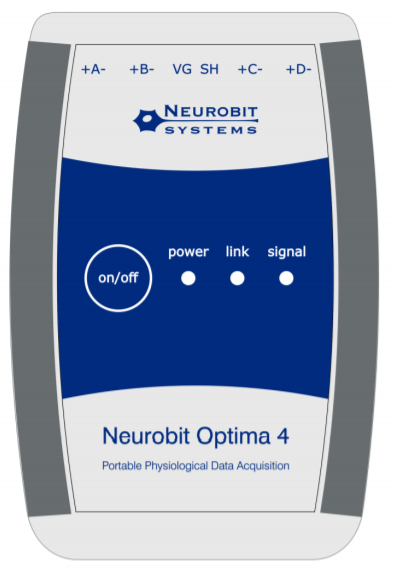
\includegraphics[width=0.3\linewidth]{images/neurobit_optima.png}
	\caption{Urządzenie Neurobit Optima, źródło: \cite{neurobit_manual}}
	\label{fig:neurobit}
\end{figure}

W kontekście platform do pomiarów sygnałów fizjologicznych w~informatyce afektywnej można zauważyć wzrost zainteresowania urządzeniami nasobnymi~\cite{wearable_sensors_2018}. Ich wyraźną zaletą jest rozmiar i~przenośność, dzięki czemu ruchy użytkownika nie są w~żadnym stopniu ograniczone. Najbardziej rozpowszechnionym, a~jednocześnie jednym z~tańszych rozwiązań, są inteligentne opaski, takie jak Xiaomi Mi Band czy Microsoft Band~\cite{wearable_sensors_2018}. Oba z~wymienionych urządzeń posiadają wbudowany optyczny sensor pulsu~\cite{miband_manual,microsoft_band_factsheet}, drugie natomiast posiada także sensor do pomiaru reakcji elektrodermalnej~\cite{microsoft_band_factsheet}. Inną, mniej popularną opaską, jest Empatica E4, która poza sensorami dostępnymi w~Xiaomi Mi Band i~Microsoft Band posiada sensor do pomiaru temperatury skóry~\cite{empatica_manual}. Warto wspomnieć też o~wbudowanych w~urządzenia sensorach ruchu używanych między innymi do zliczania kroków mogących posłużyć jako sygnał pośredni, na podstawie którego można wykryć poziom aktywności użytkownika. Niestety ogromną wadą inteligentnych opasek jest ogromna niedokładność pomiarów w~porównaniu do odczytów ze sprzętów klasy medycznej. Odczyty z~opasek charakteryzują się odczytami mocno odbiegającymi od pomiarów wykonanych przy pomocy sprzętu medycznego~\cite{wearable_sensors_2018,accuracy_of_wearables_hr}.

Innymi urządzeniami nasobnymi charakteryzującymi się większą dokładnością, do których często porównuje się odczyty z~innych urządzeń do pomiaru pracy serca~\cite{wearable_sensors_2018,accuracy_of_wearables_hr}, są monitory tętna Garmin HRM-Run oraz Polar H10. W~przeciwieństwie do optycznego sensora wbudowanego w~inteligentne opaski są one wyposażone w~suche elektrody wbudowane w~pasek zakładany na klatkę piersiową\cite{polar_manual,garmin_manual}. Jest to rozwiązanie, które nie jest inwazyjne dla użytkownika, a~jednocześnie pozwala na dokładny pomiar pracy serca. Ważną zaletą obu urządzeń jest nie tylko wsparcie dla standardu Bluetooth, ale także dla protokołu ANT+ wykorzystywanego w~coraz większej liczbie urządzeń do pomiarów aktywności użytkownika\footnote{\textit{https://www.thisisant.com/directory}}, do którego twórcy udostępniają również gotowe implementacje interfejsów do odczytywania pomiarów, dzięki którym w~prosty sposób możliwe jest zbudowanie aplikacji interpretujących wysyłane dane.

Rozwiązaniem będącym pomostem między kosztownymi platformami medycznymi a~często niedokładnymi urządzeniami nasobnymi jest platforma BITalino (r)evolution kit~\cite{bitalino_documentation}. Jest to urządzenie modułowe, składające się z~płytki stanowiącej rdzeń urządzenia, do której mogą zostać podpięte oddzielne moduły do pomiarów sygnałów fizjologicznych (rys. \ref{fig:bitalino}). Na liście dostępnych sensorów znajdują się te odpowiadające za pomiar akcji serca, reakcji elektrodermalnej skóry, czynności ruchowej mięśni oraz aktywności mózgu. Każdy z~modułów może zostać podłączony do dowolnego kanału urządzenia, natomiast pomiary odbywają się poprzez podłączenie do drugiej strony modułów kabli, na których końcu znajdują się elektrody. Co więcej, poza modułami służącymi do pomiaru reakcji fizjologicznych użytkownika, na liście dostępnych segmentów znajdują się także akcelerometr, sensor światła, dioda LED, brzęczyk, oraz przycisk, które mogą posłużyć do odczytu pomiarów pośrednich czy informowania użytkownika o~zdarzeniach. Dzięki temu platforma BITalino może służyć nie tylko jako urządzenie wykorzystywane do pomiarów, ale również do interakcji z~grą. Bardzo dużą zaletą BITalino z~perspektywy informatyki afektywnej jest dostępność narzędzi przygotowanych przez twórców, a~także ogromna ilość implementacji interfejsów do komunikacji z~urządzeniem. Twórcy na swojej stronie udostępniają biblioteki dla wielu popularnych języków programowania takich jak Python, C\# czy Java, oraz konkretne implementacje z~przykładami dla środowisk takich jak silnik do gier Unity. Dodatkowym plusem jest fakt, że większość tych implementacji jest oprogramowaniem otwartym, w~związku z~czym mogą być one rozszerzane i~naprawiane przez społeczność korzystającą z~platformy.

\begin{figure}
	\centering
	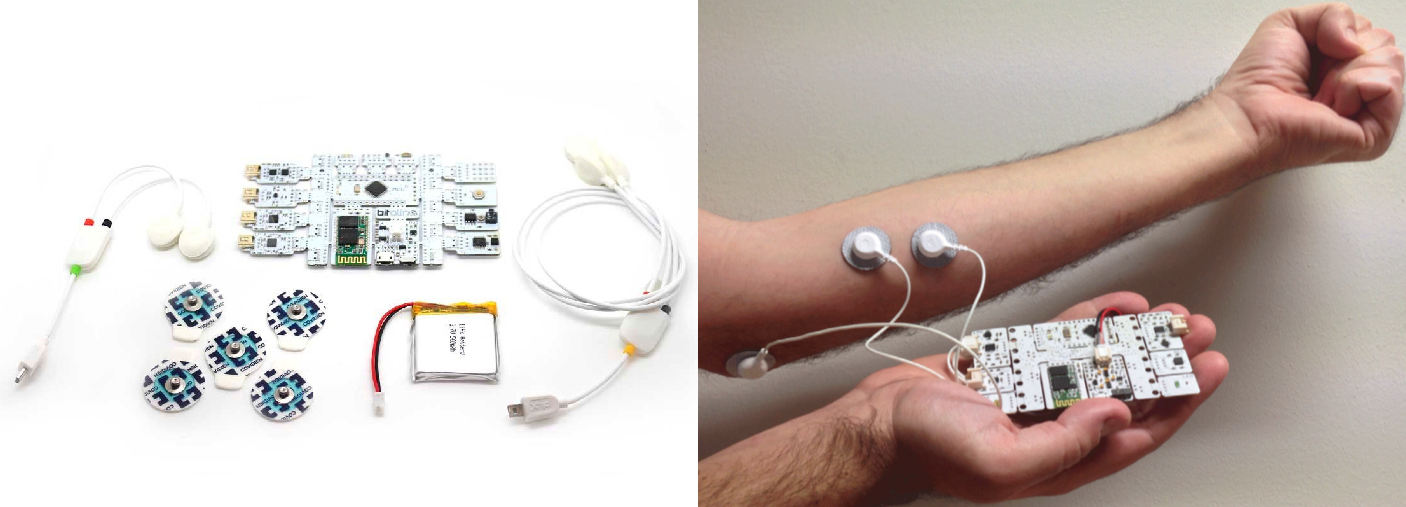
\includegraphics[width=0.9\linewidth]{images/bitalino_emg.png}
	\caption{BITalino (r)evolution kit oraz przykład podłączenia sensora do pomiaru ruchu mięśni, źródło: \cite{neurobit_manual}}
	\label{fig:bitalino}
\end{figure}

Do wspomnianej na początku drugiej kategorii urządzeń, z~których możliwe jest odczytanie sygnałów pośrednich wykorzystanych do określenia stanu użytkownika, można przede wszystkim zaliczyć sprzęty wykorzystywane przez graczy. Mowa tutaj między innymi o~myszkach, klawiaturach czy padach, z~których możliwe jest odczytanie intensywności kliknięć lub odczyt szybkości poruszania myszką na podstawie jej pozycji na ekranie~\cite{measuring_emotion_from_gamepad}. Szczególną uwagę należy poświęcić padowi Dualshock 4 od firmy Sony, który w~przeciwieństwie do większości spopularyzowanych kontrolerów do gier posiada wbudowany akcelerometr oraz żyroskop, które mogą posłużyć jako dodatkowe źródło informacji do określenia stanu emocjonalnego użytkownika~\cite{dualshock_specification}. Niestety ze względu na umowy licencyjne oprogramowanie umożliwiające odczyt tych parametrów z~pada, jest płatne, co można zaliczyć jako wadę tego rozwiązania z~perspektywy twórcy aplikacji wykorzystującej funkcjonalności Dualshocka.

\section{Możliwe mechanizmy do rozpoznawania emocji}
Opis modeli predykcji (random forest, extra trees, SVM, sieci neuronowe), krótko
\section{Narzędzia do budowy gier}
Tworzenie gier komputerowych jest złożonym procesem, wymagającym pracy w~ramach wielu dziedzin naukowych. W~przypadku przygotowywania wysokobudżetowych produkcji przy pracy nad nimi potrafi pracować nawet kilkaset osób. Od projektantów poziomów, przez osoby zajmujące się przygotowaniem sceny fabularnej, grafików, kompozytorów muzyki aż po twórców oprogramowania, którzy łączą wcześniej przygotowane elementy w~jedną całość. To właśnie ci ostatni odpowiadają za ostateczną wersję gry, jej wygląd oraz optymalizację. 

Programiści tworzący końcową wersję gry, podczas tworzenia oprogramowania odpowiadającego za poszczególne jej elementy, muszą wziąć pod uwagę to, z~jakim rodzajem gry mają do czynienia. Każdy z~gatunków gier charakteryzuje się konkretnymi wymaganiami, które programista musi jak najlepiej odwzorować w~tworzonym kodzie gry. Dla przykładu gra wojenna powinna charakteryzować się balistyką pocisków oprogramowaną za pomocą wzorów fizycznych, realistycznym biegiem bohatera, który ma określony poziom wytrzymałości, czy chociażby skutkami wybuchu granatu przedstawionymi jako uruchomione w~odpowiednim momencie elementy dźwiękowe i~graficzne. W~ostatnich latach duzą popularnością cieszą się gry z~gatunku Battle Royale~\cite{network_traffic_moll}, w~których kilkudziesięciu graczy ściera się ze sobą w~rozgrywce wieloosobowej. W~przypadku takich gier programiści muszą zwracać uwagę nie tylko na elementy związane z~rozgrywką, ale także na jak najdokładniejszą synchronizację klientów gry z~serwerem.

Ilość oraz złożoność elementów, które muszą zostać uwzględnione w~kodzie gry, powoduje, że stworzenie jej wyłącznie przy pomocy języków programowania jest niemal niemożliwe. Właśnie w~takim celu powstają oprogramowania nazywane silnikami do tworzenia gier. Umożliwiają one obsługę sterowania, grafiki, animacji, interakcji między obiektami, a~nawet sztucznej inteligencji, która może być jednym z~elementów gry. Silniki zwykle są dostępne w~formie środowisk programistycznych, które wprowadzają ułatwienia do zarządzania wcześniej wymienionymi elementami, jednocześnie przy tym nie rezygnując z~możliwości języków programowania. 

Istnieje mnóstwo silników do tworzenia gier, jednak większość z~nich stanowią rozwiązania wykorzystywane jedynie w~obrębie danej firmy, która na potrzeby gry lub całej serii stworzyła silnik spełniający wymagania i~usprawniający proces tworzenia gier produkowanych przez daną spółkę. Przykładem może być rozwijany od lat IW engine, przy pomocy którego powstała seria gier Call of Duty. Z~tego właśnie powodu większość publikacji naukowych na temat gier komputerowych oparta jest o~darmowe silniki do gier. Kilka z~takich rozwiązań omówiono poniżej, zwracając uwagę na popularność, funkcje dostępne w~danym środowisku, języki, w~których można tworzyć aplikacje oraz na jakie platformy można wydać gry stworzone przy pomocy danego silnika.

\subsection{Godot}
Godot~\cite{godot_documentation} jest silnikiem umożliwiającym tworzenie gier na platformy takie jak Windows, macOS czy Linux, a~także na środowiska mobilne oraz webowe. Dużą zaletą Godota jest mały rozmiar edytora oraz dostępność na większość popularnych systemów operacyjnych. Skrypty oprogramowujące mechaniki gry mogą być tworzone przy pomocy języków C\#, C++, oraz wysokopoziomowego języka GDScript przygotowanego specjalnie dla tej platformy. Alternatywnym rozwiązaniem do tworzenia logiki gry są także skrypty wizualne (ang. \textit{visual scripting}) polegające na budowaniu kodu przy pomocy gotowych bloków, które będą zrozumiałe nie tylko dla programistów, ale również dla grafików czy animatorów. Dużym plusem, szczególnie dla osób, które dopiero zaczynają pracę z~Godotem, jest liczba przykładowych projektów, nie tylko w~formie gotowych gier, ale również pojedynczych elementów, takich jak sposoby padania światła czy to, w~jaki sposób stworzyć realistyczną wodę w~grze. 

\begin{figure}[h]
	\centering
	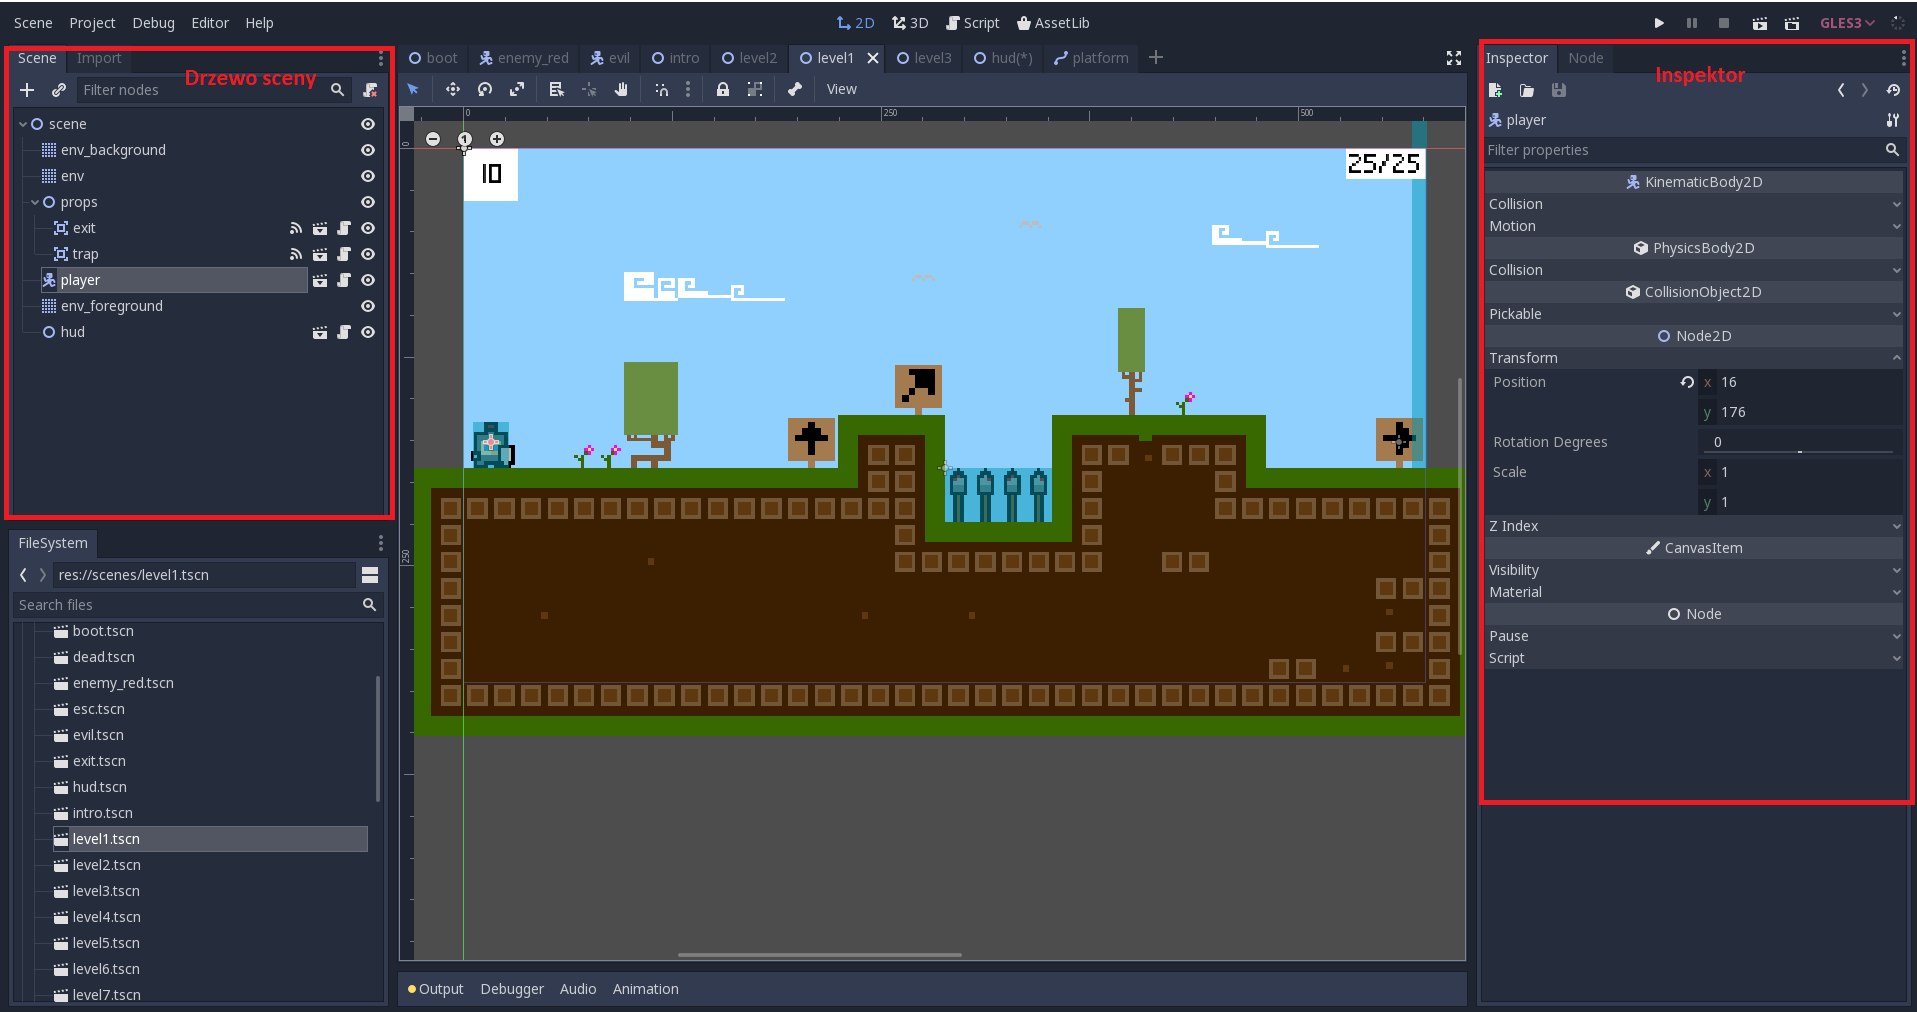
\includegraphics[width=0.9\linewidth]{images/godot_interface.png}
	\caption{Interfejs silnika Godot, po lewej stronie widać drzewo aktualnej sceny, źródło: opracowanie własne na podstawie~\cite{godot_documentation}}
	\label{fig:godot_interface}
\end{figure}

Projektowanie gier przy pomocy silnika Godot opiera się na budowaniu poszczególnych obiektów nazywanych scenami, które mogą następnie być łączone ze sobą na kolejnych scenach. Dzięki temu kolejne poziomy, a~nawet cały projekt mogą ostatecznie być opisane w~formie grafu powiązań. Dzięki takiemu rozwiązaniu projekty przygotowane przy pomocy Godota są proste w~utrzymaniu podczas wspólnej pracy wielu osób. Każdy programista może w~danej chwili zająć się oddzielną sceną, nie powodując konfliktów z~elementami przygotowanymi przez inne osoby.

\subsection{Unity}
Unity jest silnikiem umożliwiającym tworzenie gier na o~wiele większą liczbę platform niż Godot~\cite{unity_manual}. Poza opisanymi wcześniej Windowsem, Linuxem, macOS'em oraz platformami mobilnymi i~webowymi, przy pomocy Unity można tworzyć gry na konsole współczesnej generacji oraz okulary wirtualnej i~rozszerzonej rzeczywistości. Sama platforma jest dostępna na systemy Windows oraz Mac, a~od niedawna twórcy starają się dostosować ją także na dystrybucje oparte o~jądro Linux. 

Tworzenie gier w~środowisku Unity polega na tworzeniu obiektów, do których przypisane są konkretne właściwości w~zależności od rodzaju stworzonego obiektu. Do każdego z~takich elementów mogą również zostać przypisane skrypty odpowiadające za logikę działania obiektu, które tworzone są przy pomocy języka C\#. W~momencie tworzenia niniejszej pracy twórcy zapowiedzieli także dodanie skryptów wizualnych, co stanowi alternatywę dla osób niezaznajomionych z~programowaniem lub też z~samym językiem. Przygotowane obiekty są umieszczane w~środowisku gry nazywanym sceną. Interfejs Unity pozwala na bardzo proste manewrowanie pomiędzy obiektami znajdującymi się na scenie, zarządzenie ich parametrami oraz powiązaniami między obiektami.

\begin{figure}[h]
	\centering
	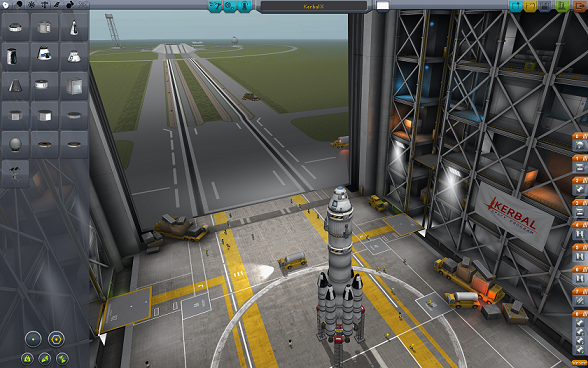
\includegraphics[width=0.7\linewidth]{images/kerbal_space_program.png}
	\caption{Kerbal Space Program, jedna z~najpopularniejszych gier stworzonych przy pomocy silnika Unity, źródło:~\cite{kerbal_your_enthusiasm}}
	\label{fig:kerbal_spaów wysokopoziomowych.ce_program}
\end{figure}

Unity jest obecnie jedną z~najpopularniejszych platform do tworzenia gier komputerowych. Przy jego pomocy powstało wiele znanych na świecie produkcji takich jak gry karciane Hearthstone i~Gwint, a~także gra symulacyjna Kerbal Space Program (rys. \ref{fig:kerbal_space_program}). Popularność ta przejawia się przede wszystkim w~postaci ogromnej liczby poradników dostępnych w~sieci, a~także aktywnej społeczności, która stale komunikuje się między sobą w~celu rozwiązania problemów występujących podczas tworzenia gier komputerowych. Dzięki temu, poza standardową dokumentacją, która także jest mocno rozbudowana, użytkownik ma dostęp do dodatkowych informacji uzyskanych od bardziej doświadczonych programistów. Cechą platformy, która mogła wpłynąć na jej popularność, jest także specjalnie przygotowany sklep zawierający zarówno płatne, jak i~darmowe dodatki rozszerzające możliwości silnika lub po prostu ułatwiające pracę przy konkretnym gatunku gry.

\subsection{Unreal Engine}
Unreal Engine jest silnikiem, który przez wiele lat był wykorzystywany jedynie do tworzenia dużych, komercyjnych gier. Do momentu wydania wersji trzeciej, projektowanie gier przy jego pomocy było ograniczone odpłatną licencją~\cite{unreal_manual}. Dopiero w~roku 2009 twórcy silnika wydali oprogramowanie Unreal Development Kit, będące darmową wersją trzeciej wersji silnika, z~uszczuploną bazą gotowych modeli oraz bez dostępu do kodu źródłowego silnika~\cite{udk_manual}. Dopiero kilka lat po wydaniu Unreal Engine 4 twórcy zdecydowali się na udostępnienie pełnego silnika za darmo. 

Spośród opisywanych rozwiązań, Unreal Engine jest najbardziej rozbudowanym. Podobnie do Unity umożliwia tworzenie gier na większość dostępnych platform, w~tym także okularów wirtualnej rzeczywistości. Językiem programowania wykorzystywanym do projektowania gier w~tym silniku jest C++, co można traktować jako wadę, ponieważ jest to język trudny i~wymagający dużo czasu na opanowanie. Z~drugiej strony jednak gry napisane przy pomocy C++ potrafią działać szybciej i~płynniej od rozwiązań stworzonych przy pomocy języków wysokopoziomowych. Ogromną zaletą silnika, która wyróżnia go na tle innych rozwiązań, jest dostęp do kodu źródłowego. Dzięki temu, twórcy gier mogą dostosować, a~nawet rozszerzyć możliwości platformy. 

Dla osób niepracujących z~kodem Unreal Engine udostępnia rozbudowany interfejs, pozwalający na stworzenie gry bez konieczności pisania kodu. Podobnie jak w~przypadku Unity, projekt gry składa się z~powiązanych ze sobą scen, tutaj nazywanych poziomami. Na każdej ze scen umieszczone są obiekty, nazywane aktorami, pomiędzy którymi zaprogramowane są interakcje specyficzne dla danej sceny. Osoba tworząca grę może zaprogramować jej logikę przy pomocy skryptów wizualnych. Tutaj warto opisać kolejny atut wyróżniający ten silnik na tle innych, którym jest możliwość korzystania z~edytora przy pomocy okularów wirtualnej rzeczywistości podczas tworzenia gier na tę platformę (rys. \ref{fig:unreal_vr_editor}). Twórca dostaje możliwość dokładnego zaprojektowania świata gry, patrząc na nią od razu z~perspektywy gracza. 

\begin{figure}
	\centering
	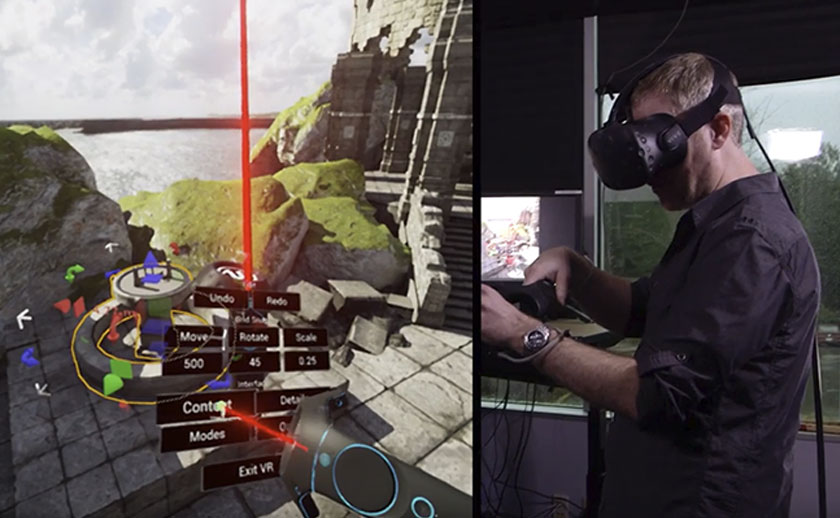
\includegraphics[width=0.7\linewidth]{images/unreal_vr_editor.jpg}
	\caption{Interfejs edytora Unreal Engine w~wirtualnej rzeczywistości, źródło:~\cite{unreal_manual}}
	\label{fig:unreal_vr_editor}
\end{figure}

Unreal Engine jest obecnie drugą, tuż po Unity, najpopularniejszą otwartą platformą do gier. Przewaga Unity wynika tutaj nie z~większych możliwości silnika, ale z~jego otwartości od początku istnienia. Ponieważ jednak przez wiele lat Unreal Engine był wykorzystywany głównie w~rozwiązaniach komercyjnych, posiada rozbudowaną, złożoną dokumentację, która opisuje każdy fragment możliwości edytora. Po udostępnieniu darmowej wersji oprogramowania pojawiła się także duża ilość materiałów na temat tworzenia gier przy pomocy Unreal Engine, a~także urosła społeczność twórców gier, którzy wykorzystują ten silnik i~wymieniają się między sobą cennymi informacjami. 
